\chapter{Resultados}\label{capit:cap5}
\vspace{-2.0325ex}%
\noindent
\rule{\textwidth}{0.5pt}
\vspace{-5.5ex}% 
\newcommand{\pushline}{\Indp}% Indent puede ir o no :p

En este capítulo se presentan los resultados de las pruebas realizadas al sistema. El desempeño del sistema es evaluado con respecto al error de clasificación.   

Los experimentos y el sistema propuesto fue implementado en una computadora de escritorio Dell con un procesador Intel(R) Xeon(R) CPU E5-1603, 16GB de memoria RAM, Windows 7 de 64 bits. La implementación del sistema se realizó en C\# utilizando Emgu 2.410 \footnote{\url{http://www.emgu.com/wiki/index.php/Main\_Page}} un wrapper de OpenCV\footnote{\url{http://opencv.org/}}. 

Para analizar la tasa de precisión de reconocimiento del sistema propuesto se realizaron varios experimentos en distintas circunstancias. Por ejemplo se analizó el rendimiento del sistema a tres diferentes distancias $70$, $80$, $90$ $cm.$ del Kinect frontal. También en diferentes circunstancias de iluminación, con iluminación estándar, media y sin iluminación. 


Se utilizaron imágenes reales capturadas por los sensores de profundidad de $640 \times 480$ pixeles. Las imágenes son de 5 personas distintas, realizando los gestos de puño y el de palma de la mano con los dedos separados, para los gestos estáticos. Para los gestos dinámicos se tomaron los gestos de $3$ personas cada una de ellas realizaron los gestos estáticos anteriores en movimiento.   

En las secciones siguientes se explica cada experimento y resultados de estos.  

\section{Experimentos de gestos estáticos}\label{TestStaticGestures}  

La evaluación del sistema en cuanto al reconocimiento de los gestos estáticos, se determino conforme al resultado de los experimentos realizados en circunstancias de iluminación, (estándar, media, baja). En cada conjunto de experimentos se tomo en cuenta la distancia, ya que en cada grupo se analizaron tres distancias, $70$, $80$, $90$ $cm$.  

Se analizaron dos gestos estáticos la palma de la mano con los dedos separados, Gesto 1 y el puño, Gesto 2, de $5$ usuarios distintos. Para cada experimento se escogió al azar $200$ imágenes de cada gesto del conjunto de las imágenes capturadas. 

Enseguida se presentan los resultados de cada experimento realizado.

\subsection{Experimentos con iluminación} 
Para este experimento las imágenes se capturaron en un laboratorio con iluminación estándar,como la que se muestra en la figura \ref{fig:LabIluminado}.

\begin{figure}[h!]
\begin{center} 
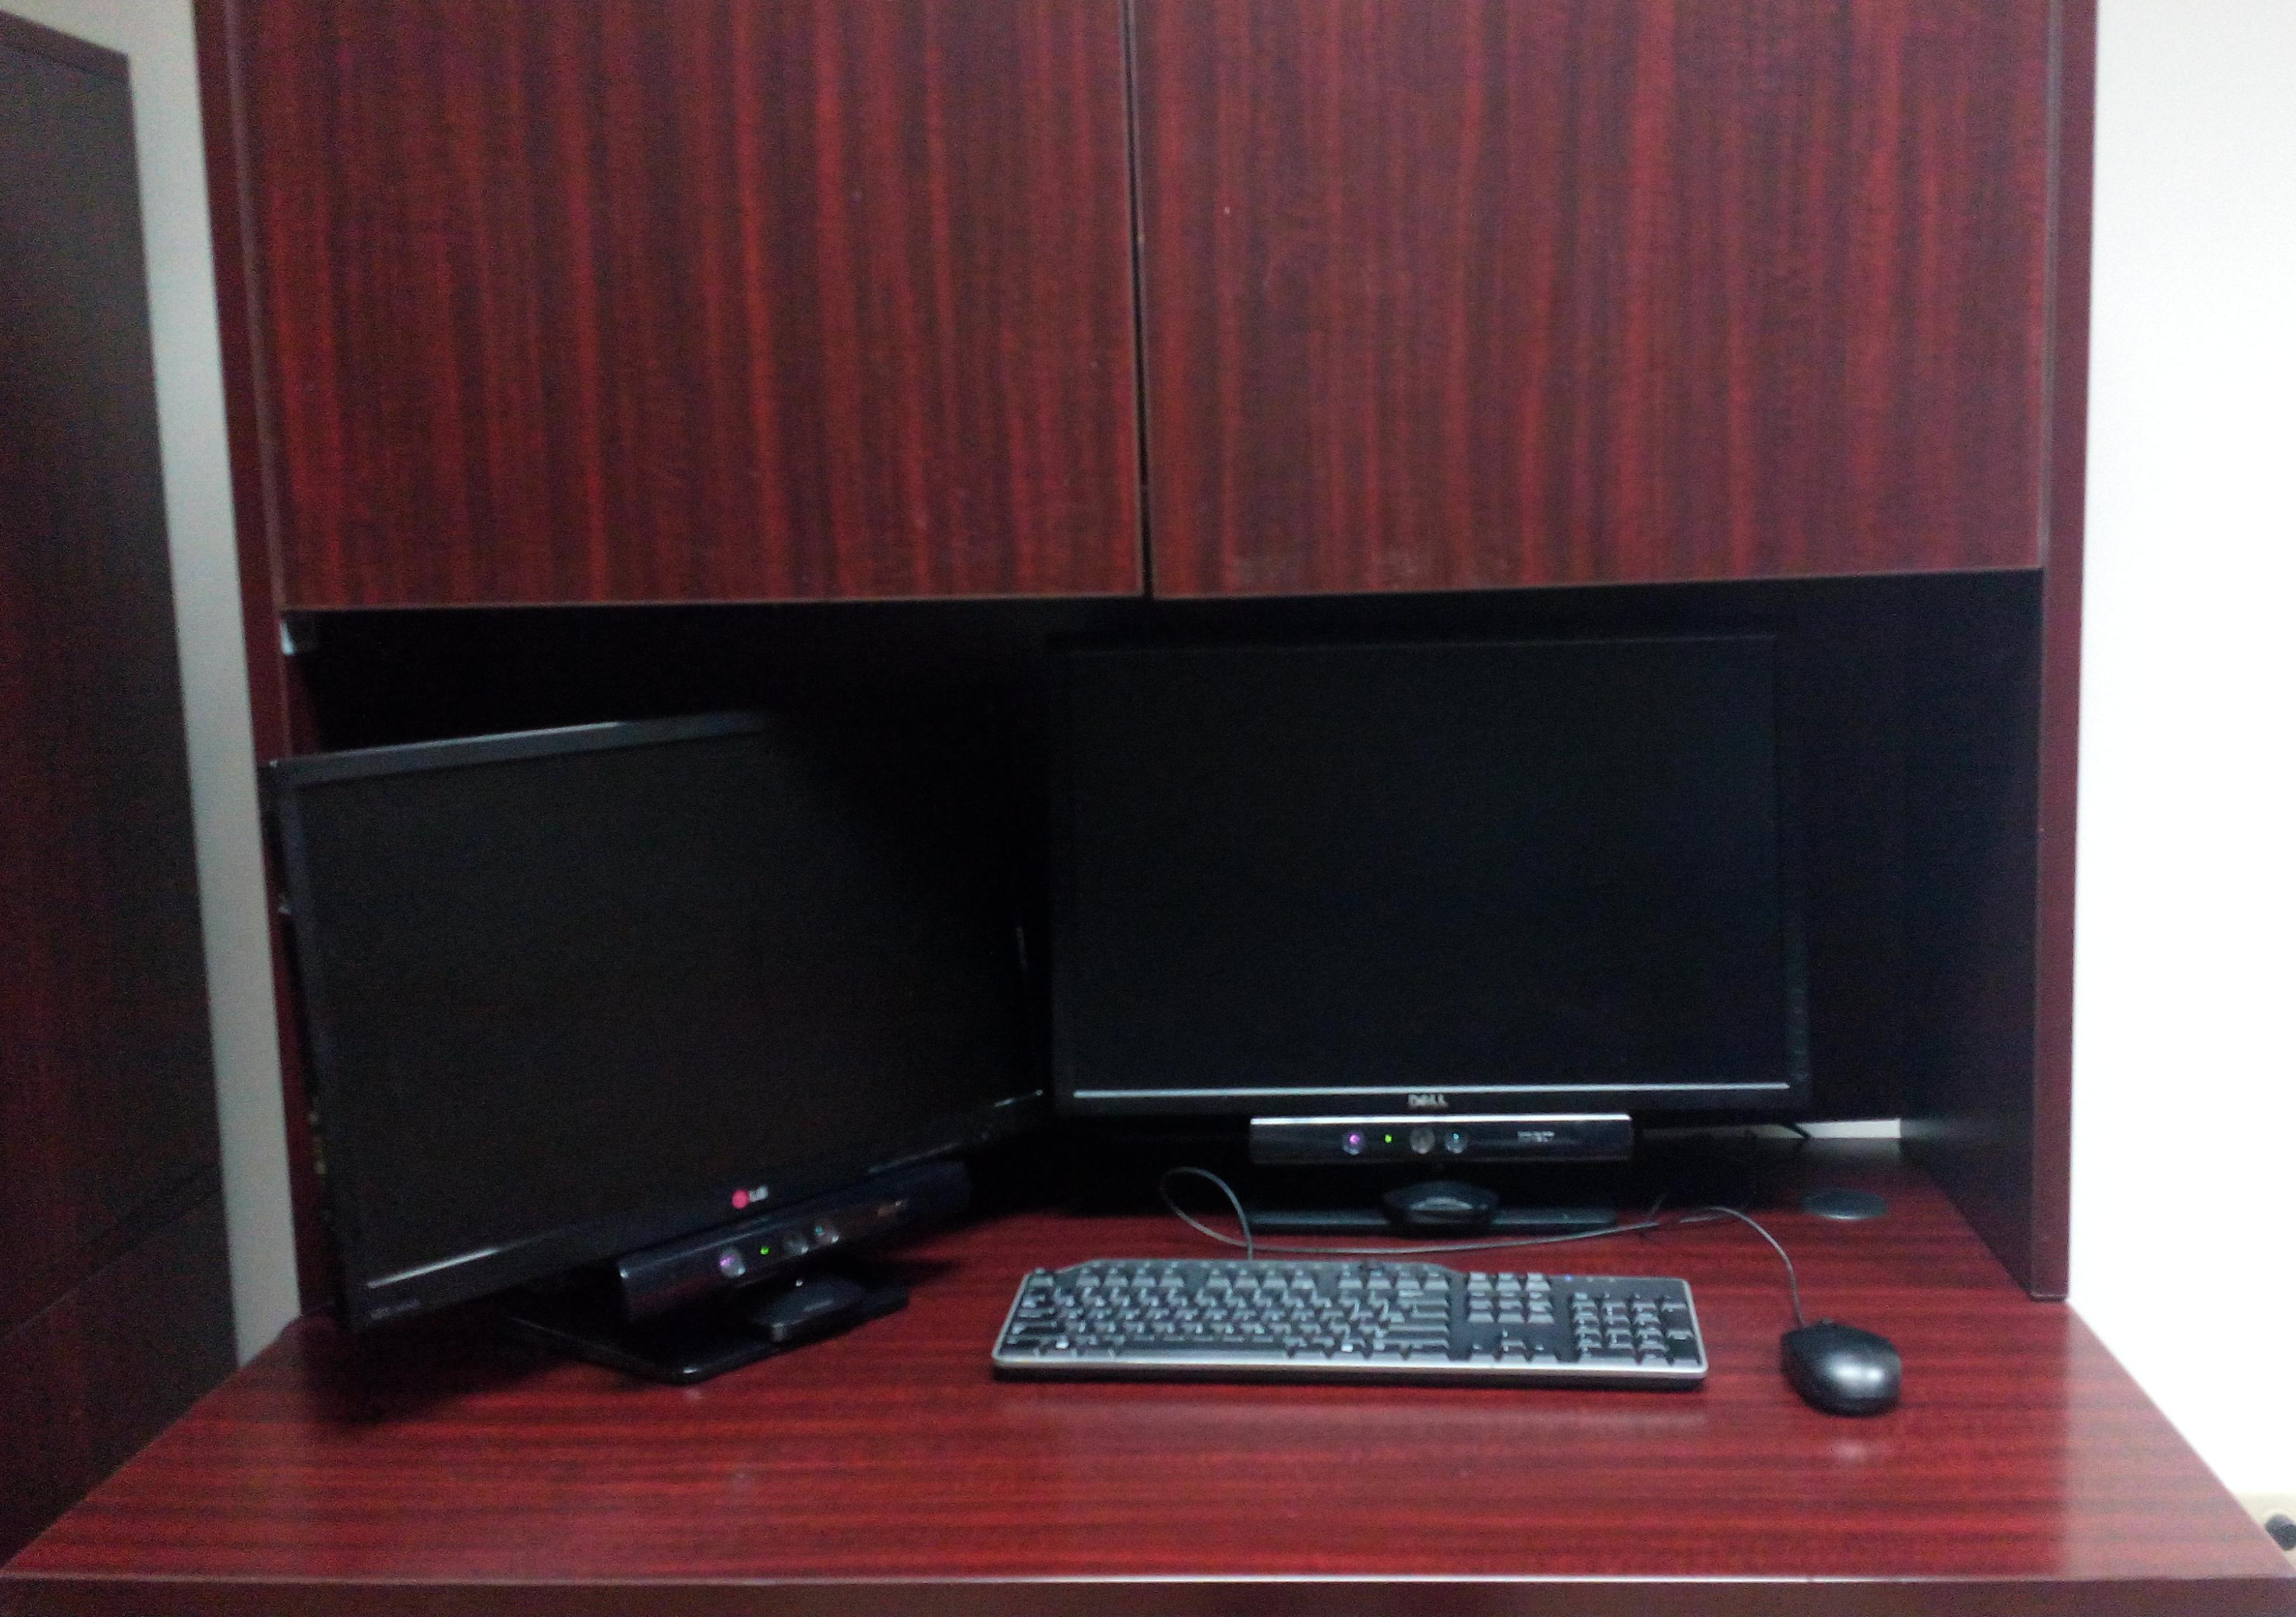
\includegraphics[scale=0.09]{./Figures/iluminacion.jpg}
\end{center}
\caption{Laboratorio en condiciones estándar de iluminación.}
\label{fig:LabIluminado}
\end{figure} 

En el primer experimento el usuario esta a una distancia de $70$ $cm.$ del Kinect frontal. Se muestra un ejemplo de las imágenes obtenidas de un usuario, para las imágenes de los demás usuarios ver el apéndice . En la tabla se encuentran los resultados del reconocimiento de los dos gestos.  

\begin{figure}[h!]
\centering
\subfigure[Gesto 1 vista desde el Kinect frontal]{
\includegraphics[scale=.3]{./Figures/pusheen}\label{fig:iluminacion70:1}}
\subfigure[Gesto 1 viata desde el Kinect lateral]{
\includegraphics[scale=.3]{./Figures/pusheen}\label{fig:iluminacion70:2}}
\subfigure[Gesto 2 vista desde Kinect frontal]{
\includegraphics[scale=.3]{./Figures/pusheen}\label{fig:iluminacion70:3}}
\subfigure[Gesto 2 vista desde Kinect lateral]{
\includegraphics[scale=.3]{./Figures/pusheen}\label{fig:iluminacion70:4}}
\caption{Ejemplo de la imagenes capturadas a una distancia de $70$ $cm$.} \label{fig:iluminacion70}
\end{figure}


\begin{table}[h!] 
\begin{center}
\begin{tabular}{ r || c | c |} 
 
        & Gesto 1 & Gesto 2 \\ \hline \hline  
Gesto 1 & 183     &  17     \\ \hline  
Gesto 2 & 11      & 189     \\   

\end{tabular}
\end{center} 
\caption{Matriz de confusión}
\end{table}


En el segundo experimento el usuario esta a una distancia de $80$ $cm.$ del Kinect frontal. Se muestra un ejemplo de las imágenes obtenidas de un usuario. En la tabla se encuentran los resultados del reconocimiento de los dos gestos.   

\begin{figure}[h!]
\centering
\subfigure[Gesto 1 vista desde el Kinect frontal]{
\includegraphics[scale=.3]{./Figures/pusheen}\label{fig:iluminacion80:1}}
\subfigure[Gesto 1 viata desde el Kinect lateral]{
\includegraphics[scale=.3]{./Figures/pusheen}\label{fig:iluminacion80:2}}
\subfigure[Gesto 2 vista desde Kinect frontal]{
\includegraphics[scale=.3]{./Figures/pusheen}\label{fig:iluminacion80:3}}
\subfigure[Gesto 2 vista desde Kinect lateral]{
\includegraphics[scale=.3]{./Figures/pusheen}\label{fig:iluminacion80:4}}
\caption{Ejemplo de la imagenes capturadas a una distancia de $80$ $cm$.} \label{fig:iluminacion80}
\end{figure}




En el tercer experimento el usuario esta a una distancia de $90$ $cm.$ del Kinect frontal. Se muestra un ejemplo de las imágenes obtenidas de un usuario. En la tabla se encuentran los resultados del reconocimiento de los dos gestos.    

\begin{figure}[h!]
\centering
\subfigure[Gesto 1 vista desde el Kinect frontal]{
\includegraphics[scale=.3]{./Figures/pusheen}\label{fig:iluminacion90:1}}
\subfigure[Gesto 1 viata desde el Kinect lateral]{
\includegraphics[scale=.3]{./Figures/pusheen}\label{fig:iluminacion90:2}}
\subfigure[Gesto 2 vista desde Kinect frontal]{
\includegraphics[scale=.3]{./Figures/pusheen}\label{fig:iluminacion90:3}}
\subfigure[Gesto 2 vista desde Kinect lateral]{
\includegraphics[scale=.3]{./Figures/pusheen}\label{fig:iluminacion90:4}}
\caption{Ejemplo de la imagenes capturadas a una distancia de $90$ $cm$.} \label{fig:iluminacion70}
\end{figure}



\subsection{Experimentos con iluminación media} 
Para el conjunto de estos experimentos, las imágenes se capturaron en un laboratorio con iluminación media, como la que se muestra en la figura. A tres distancias $70$, $80$ y $90$ $cm$.  

\begin{figure}[h!]
\begin{center} 
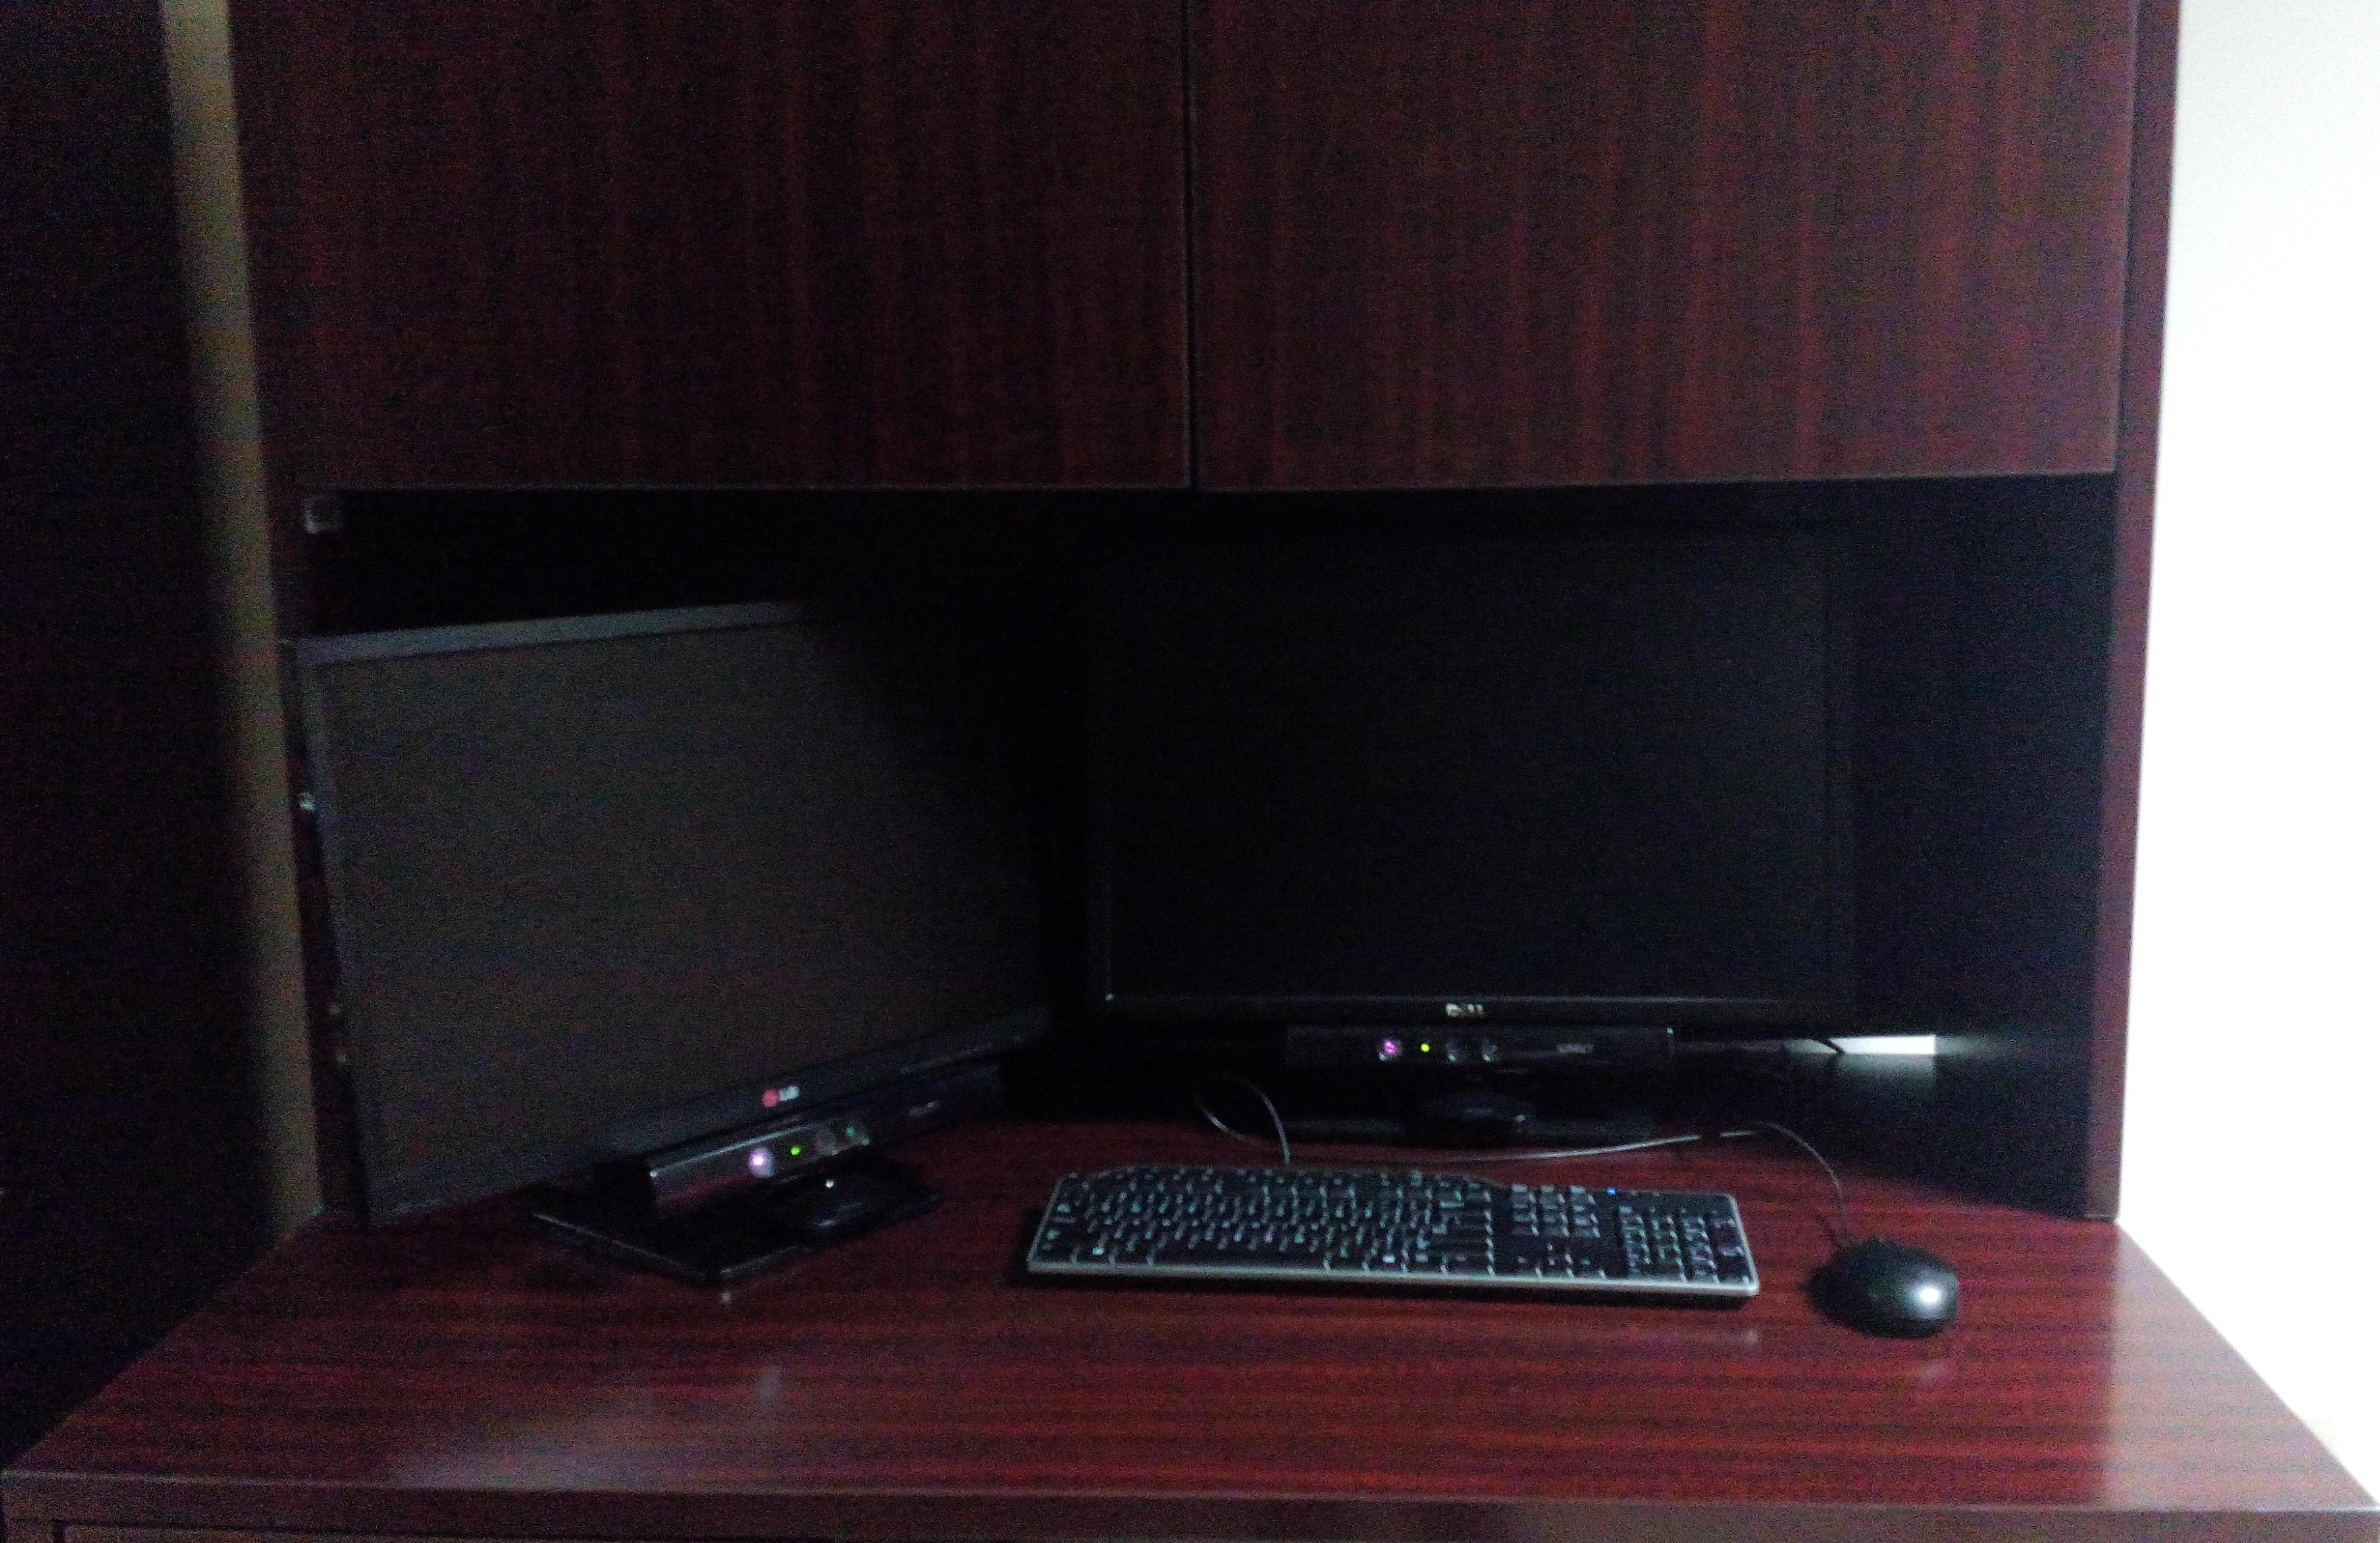
\includegraphics[scale=0.09]{./Figures/mediailuminacion.jpg}
\end{center}
\caption{Laboratorio en condiciones con iluminación media.}
\label{fig:LabMedioIluminado} 
\end{figure}  

En el primer experimento el usuario esta a una distancia de $70$ $cm.$ del Kinect frontal. Se muestra un ejemplo de las imágenes obtenidas de un usuario. En la tabla se encuentran los resultados del reconocimiento de los dos gestos.  

\begin{figure}[h!]
\centering
\subfigure[Gesto 1 vista desde el Kinect frontal]{
\includegraphics[scale=.3]{./Figures/pusheen}\label{fig:iluminacionM70:1}}
\subfigure[Gesto 1 viata desde el Kinect lateral]{
\includegraphics[scale=.3]{./Figures/pusheen}\label{fig:iluminacionM70:2}}
\subfigure[Gesto 2 vista desde Kinect frontal]{
\includegraphics[scale=.3]{./Figures/pusheen}\label{fig:iluminacionM70:3}}
\subfigure[Gesto 2 vista desde Kinect lateral]{
\includegraphics[scale=.3]{./Figures/pusheen}\label{fig:iluminacionM70:4}}
\caption{Ejemplo de la imagenes capturadas a una distancia de $70$ $cm$.} \label{fig:iluminacionM70}
\end{figure}

%\begin{tabular} { c c c }
% cell1 & cell2 & cell3 \\ 
% cell4 & cell5 & cell6 \\  
% cell7 & cell8 & cell9    
%\end{tabular}

En el segundo experimento el usuario esta a una distancia de $80$ $cm.$ del Kinect frontal. Se muestra un ejemplo de las imágenes obtenidas de un usuario. En la tabla se encuentran los resultados del reconocimiento de los dos gestos.   

\begin{figure}[h!]
\centering
\subfigure[Gesto 1 vista desde el Kinect frontal]{
\includegraphics[scale=.3]{./Figures/pusheen}\label{fig:iluminacionM80:1}}
\subfigure[Gesto 1 viata desde el Kinect lateral]{
\includegraphics[scale=.3]{./Figures/pusheen}\label{fig:iluminacionM80:2}}
\subfigure[Gesto 2 vista desde Kinect frontal]{
\includegraphics[scale=.3]{./Figures/pusheen}\label{fig:iluminacionM80:3}}
\subfigure[Gesto 2 vista desde Kinect lateral]{
\includegraphics[scale=.3]{./Figures/pusheen}\label{fig:iluminacionM80:4}}
\caption{Ejemplo de la imagenes capturadas a una distancia de $80$ $cm$.} \label{fig:iluminacionM80}
\end{figure}

%\begin{tabular} { c c c }
% cell1 & cell2 & cell3 \\ 
% cell4 & cell5 & cell6 \\  
% cell7 & cell8 & cell9    
%\end{tabular} 

En el tercer experimento el usuario esta a una distancia de $90$ $cm.$ del Kinect frontal. Se muestra un ejemplo de las imágenes obtenidas de un usuario. En la tabla se encuentran los resultados del reconocimiento de los dos gestos.    

\begin{figure}[h!]
\centering
\subfigure[Gesto 1 vista desde el Kinect frontal]{
\includegraphics[scale=.3]{./Figures/pusheen}\label{fig:iluminacionM90:1}}
\subfigure[Gesto 1 viata desde el Kinect lateral]{
\includegraphics[scale=.3]{./Figures/pusheen}\label{fig:iluminacionM90:2}}
\subfigure[Gesto 2 vista desde Kinect frontal]{
\includegraphics[scale=.3]{./Figures/pusheen}\label{fig:iluminacionM90:3}}
\subfigure[Gesto 2 vista desde Kinect lateral]{
\includegraphics[scale=.3]{./Figures/pusheen}\label{fig:iluminacionM90:4}}
\caption{Ejemplo de la imagenes capturadas a una distancia de $90$ $cm$.} \label{fig:iluminacionM90}
\end{figure}

%\begin{tabular} { c c c }
% cell1 & cell2 & cell3 \\ 
% cell4 & cell5 & cell6 \\  
% cell7 & cell8 & cell9    
%\end{tabular}


\subsection{Experimentos sin iluminación}
Para este experimento las imágenes se capturaron en un laboratorio sin iluminación, como la que se muestra en la figura.

\begin{figure}[h!]
\begin{center} 
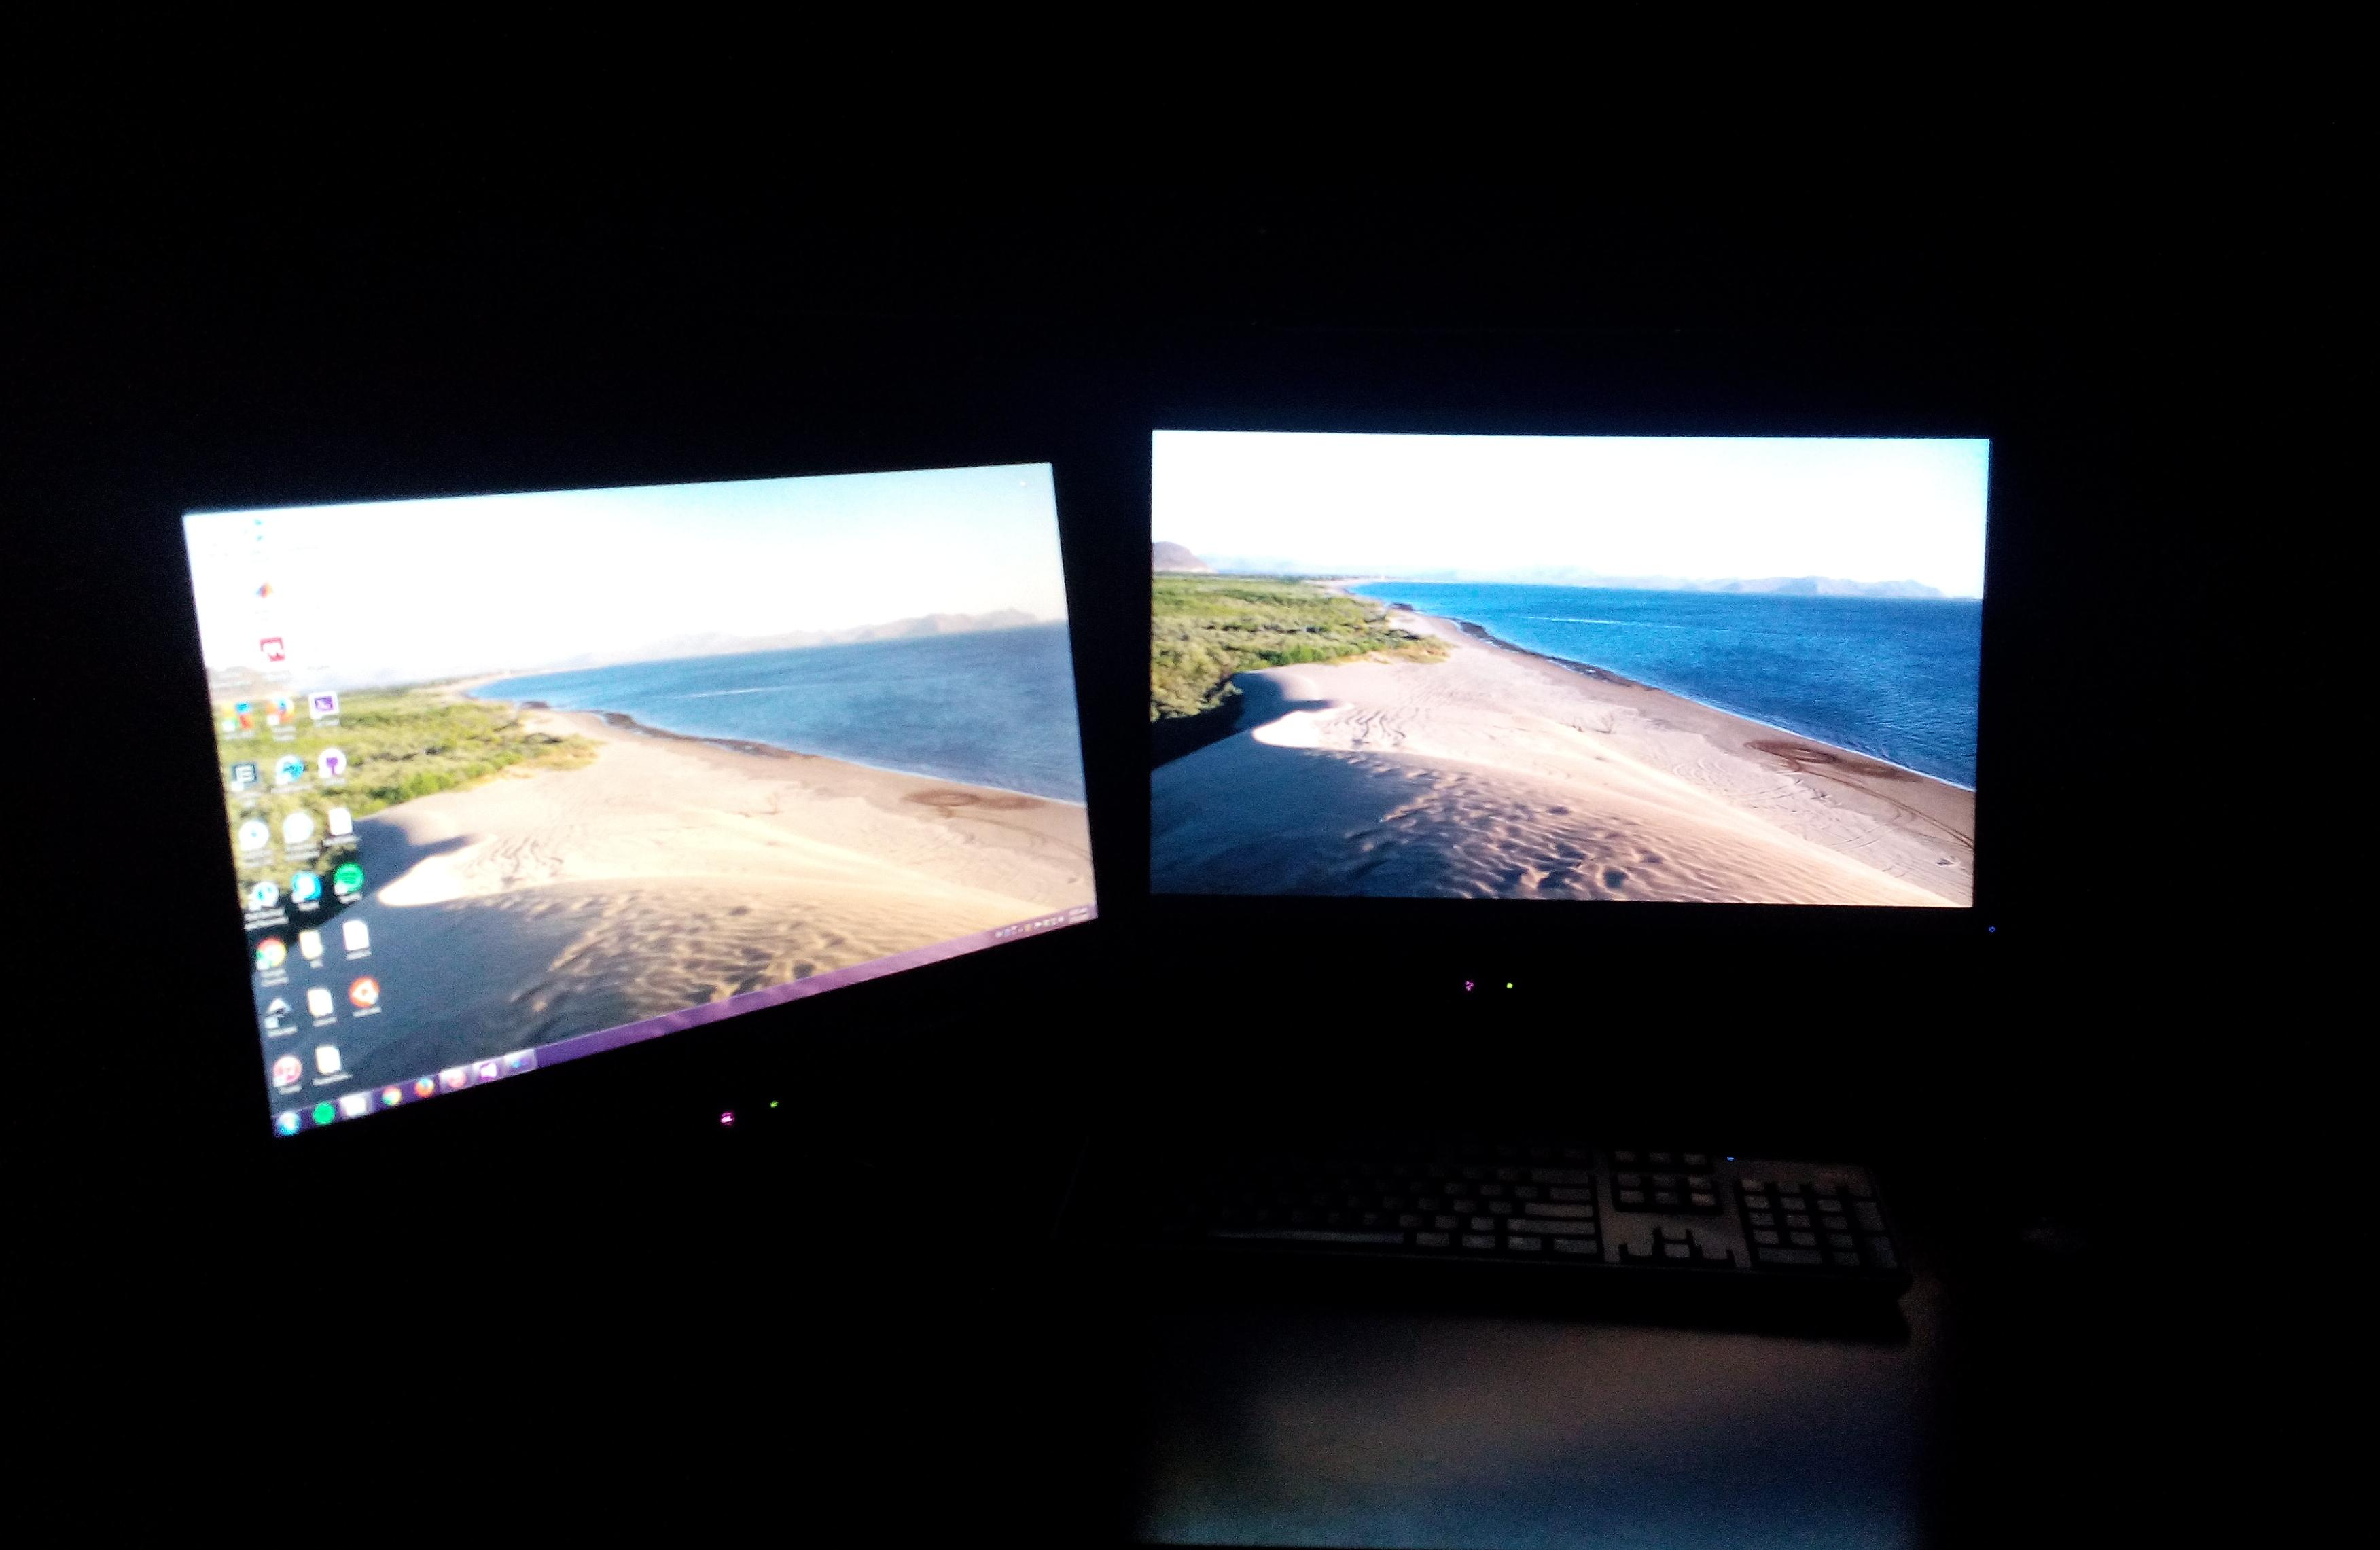
\includegraphics[scale=0.09]{./Figures/noIluminacion.jpg}
\end{center}
\caption{Laboratorio en condiciones con baja iluminación.}
\label{fig:LabNoIluminado} 
\end{figure} 

En el primer experimento el usuario esta a una distancia de $70$ $cm.$ del Kinect frontal. Se muestra un ejemplo de las imágenes obtenidas de un usuario. En la tabla se encuentran los resultados del reconocimiento de los dos gestos.  

\begin{figure}[h!]
\centering
\subfigure[Gesto 1 vista desde el Kinect frontal]{
\includegraphics[scale=.3]{./Figures/pusheen}\label{fig:iluminacionNo70:1}}
\subfigure[Gesto 1 viata desde el Kinect lateral]{
\includegraphics[scale=.3]{./Figures/pusheen}\label{fig:iluminacionNo70:2}}
\subfigure[Gesto 2 vista desde Kinect frontal]{
\includegraphics[scale=.3]{./Figures/pusheen}\label{fig:iluminacionNo70:3}}
\subfigure[Gesto 2 vista desde Kinect lateral]{
\includegraphics[scale=.3]{./Figures/pusheen}\label{fig:iluminacionNo70:4}}
\caption{Ejemplo de la imagenes capturadas a una distancia de $70$ $cm$.} \label{fig:iluminacionNo70}
\end{figure}

%\begin{tabular} { c c c }
% cell1 & cell2 & cell3 \\ 
% cell4 & cell5 & cell6 \\  
% cell7 & cell8 & cell9    
%\end{tabular}

En el segundo experimento el usuario esta a una distancia de $80$ $cm.$ del Kinect frontal. Se muestra un ejemplo de las imágenes obtenidas de un usuario. En la tabla se encuentran los resultados del reconocimiento de los dos gestos.   

\begin{figure}[h!]
\centering
\subfigure[Gesto 1 vista desde el Kinect frontal]{
\includegraphics[scale=.3]{./Figures/pusheen}\label{fig:iluminacionNo80:1}}
\subfigure[Gesto 1 viata desde el Kinect lateral]{
\includegraphics[scale=.3]{./Figures/pusheen}\label{fig:iluminacionNo80:2}}
\subfigure[Gesto 2 vista desde Kinect frontal]{
\includegraphics[scale=.3]{./Figures/pusheen}\label{fig:iluminacionNo80:3}}
\subfigure[Gesto 2 vista desde Kinect lateral]{
\includegraphics[scale=.3]{./Figures/pusheen}\label{fig:iluminacionNo80:4}}
\caption{Ejemplo de la imagenes capturadas a una distancia de $80$ $cm$.} \label{fig:iluminacionNo80}
\end{figure}

%\begin{tabular} { c c c }
% cell1 & cell2 & cell3 \\ 
% cell4 & cell5 & cell6 \\  
% cell7 & cell8 & cell9    
%\end{tabular} 

En el tercer experimento el usuario esta a una distancia de $90$ $cm.$ del Kinect frontal. Se muestra un ejemplo de las imágenes obtenidas de un usuario. En la tabla se encuentran los resultados del reconocimiento de los dos gestos.    

\begin{figure}[h!]
\centering
\subfigure[Gesto 1 vista desde el Kinect frontal]{
\includegraphics[scale=.3]{./Figures/pusheen}\label{fig:iluminacionNo90:1}}
\subfigure[Gesto 1 viata desde el Kinect lateral]{
\includegraphics[scale=.3]{./Figures/pusheen}\label{fig:iluminacionNo90:2}}
\subfigure[Gesto 2 vista desde Kinect frontal]{
\includegraphics[scale=.3]{./Figures/pusheen}\label{fig:iluminacionNo90:3}}
\subfigure[Gesto 2 vista desde Kinect lateral]{
\includegraphics[scale=.3]{./Figures/pusheen}\label{fig:iluminacionNo90:4}}
\caption{Ejemplo de la imagenes capturadas a una distancia de $90$ $cm$.} \label{fig:iluminacionNo70}
\end{figure}

%\begin{tabular} { c c c }
% cell1 & cell2 & cell3 \\ 
% cell4 & cell5 & cell6 \\  
% cell7 & cell8 & cell9    
%\end{tabular}


%:::::::::::::::::::::::::::::::::::::::::::::::::::::::::::::::::::::::::::::::::::::::::::::::::::::::::::::::::


\section{Experimentos de gestos dinámicos}\label{TestDinamicGestures} 

La evaluación del sistema en cuanto al reconocimiento de los gestos dinámicos se realizo de la siguiente forma; al igual que en los gestos estáticos se hicieron tres conjuntos de experimentos cada uno con diferentes tipos de iluminación, estándar, iluminación media y sin iluminación. En cada conjunto de experimentos se tomo en cuenta la distancia, ya que en cada grupo se analizaron tres distancias, $70$, $80$, $90$ $cm$. 

Los gestos analizados fueron dos el primero es la palma con los dedos separados, en movimiento y el segundo el puño de la mano también en movimiento. Estos gestos fueron realizados por tres usuarios distintos. Para cada experimento se analizaron $num$ cuadros por lo que se analizaron $num$ gestos y cada uno tenia una duración de $60$ cuadros.  

Enseguida se presentan los resultados de cada experimento realizado. 

\subsection{Experimentos con iluminación} 
Para este experimento las imágenes se capturaron en un laboratorio con iluminación estándar,como la que se muestra en la figura \ref{fig:LabIluminado}.

En el primer experimento el usuario esta a una distancia de $70$ $cm.$ del Kinect frontal. Se muestra un ejemplo de las imágenes obtenidas de un usuario, para las imágenes de los demás usuarios ver el apéndice . En la tabla se encuentran los resultados del reconocimiento de los dos gestos.  

\begin{figure}[h!]
\centering
\subfigure[Cuadro inicial]{
\includegraphics[scale=.3]{./Figures/pusheen}\label{fig:G1I70:1}}
\subfigure[Cuadro número 20]{
\includegraphics[scale=.3]{./Figures/pusheen}\label{fig:G1I70:2}}
\subfigure[Cuadro número 40]{
\includegraphics[scale=.3]{./Figures/pusheen}\label{fig:G1I70:3}}
\subfigure[Cuadro final]{
\includegraphics[scale=.3]{./Figures/pusheen}\label{fig:G1I70:4}}
\caption{Gesto de la palma con los dedos abiertas a $70$ $cm$.} \label{fig:G1I70}
\end{figure}

\begin{figure}[h!]
\centering
\subfigure[Cuadro inicial]{
\includegraphics[scale=.3]{./Figures/pusheen}\label{fig:G2I70:1}}
\subfigure[Cuadro número 20]{
\includegraphics[scale=.3]{./Figures/pusheen}\label{fig:G2I70:2}}
\subfigure[Cuadro número 40]{
\includegraphics[scale=.3]{./Figures/pusheen}\label{fig:G2I70:3}}
\subfigure[Cuadro final]{
\includegraphics[scale=.3]{./Figures/pusheen}\label{fig:G2I70:4}}
\caption{Gesto del puño de la mano a $70$ $cm$.} \label{fig:G2I70}
\end{figure}

%\begin{tabular} { c c c }
% cell1 & cell2 & cell3 \\ 
% cell4 & cell5 & cell6 \\  
% cell7 & cell8 & cell9    
%\end{tabular}

En el segundo experimento el usuario esta a una distancia de $80$ $cm.$ del Kinect frontal. Se muestra un ejemplo de las imágenes obtenidas de un usuario. En la tabla se encuentran los resultados del reconocimiento de los dos gestos.   

\begin{figure}[h!]
\centering
\subfigure[Cuadro inicial]{
\includegraphics[scale=.3]{./Figures/pusheen}\label{fig:G1I80:1}}
\subfigure[Cuadro número 20]{
\includegraphics[scale=.3]{./Figures/pusheen}\label{fig:G1I80:2}}
\subfigure[Cuadro número 40]{
\includegraphics[scale=.3]{./Figures/pusheen}\label{fig:G1I80:3}}
\subfigure[Cuadro final]{\includegraphics[scale=.3]{./Figures/pusheen}\label{fig:G1I80:4}}
\caption{Gesto de la palma con los dedos abiertas a $80$ $cm$.} \label{fig:G1I80}
\end{figure}

\begin{figure}[h!]
\centering
\subfigure[Cuadro inicial]{\includegraphics[scale=.3]{./Figures/pusheen}\label{fig:G2I80:1}}
\subfigure[Cuadro número 20]{\includegraphics[scale=.3]{./Figures/pusheen}\label{fig:G2I80:2}}
\subfigure[Cuadro número 40]{\includegraphics[scale=.3]{./Figures/pusheen}\label{fig:G2I80:3}}
\subfigure[Cuadro final]{\includegraphics[scale=.3]{./Figures/pusheen}\label{fig:G2I80:4}}
\caption{Gesto del puño de la mano a $80$ $cm$.} \label{fig:G2I0}
\end{figure}

%\begin{tabular} { c c c }
% cell1 & cell2 & cell3 \\ 
% cell4 & cell5 & cell6 \\  
% cell7 & cell8 & cell9    
%\end{tabular} 

En el tercer experimento el usuario esta a una distancia de $90$ $cm.$ del Kinect frontal. Se muestra un ejemplo de las imágenes obtenidas de un usuario. En la tabla se encuentran los resultados del reconocimiento de los dos gestos.    

\begin{figure}[h!]
\centering
\subfigure[Cuadro inicial]{\includegraphics[scale=.3]{./Figures/pusheen}\label{fig:G1I90:1}}
\subfigure[Cuadro número 20]{\includegraphics[scale=.3]{./Figures/pusheen}\label{fig:G1I90:2}}
\subfigure[Cuadro número 40]{\includegraphics[scale=.3]{./Figures/pusheen}\label{fig:G1I90:3}}
\subfigure[Cuadro final]{\includegraphics[scale=.3]{./Figures/pusheen}\label{fig:G1I90:4}}
\caption{Gesto de la palma con los dedos abiertas $90$ $cm$.} \label{fig:G1I90}
\end{figure}

\begin{figure}[h!]
\centering
\subfigure[Cuadro inicial]{\includegraphics[scale=.3]{./Figures/pusheen}\label{fig:G2I90:1}}
\subfigure[Cuadro número 20]{\includegraphics[scale=.3]{./Figures/pusheen}\label{fig:G2I90:2}}
\subfigure[Cuadro número 40]{\includegraphics[scale=.3]{./Figures/pusheen}\label{fig:G2I90:3}}
\subfigure[Cuadro final]{\includegraphics[scale=.3]{./Figures/pusheen}\label{fig:G2I90:4}}
\caption{Gesto del puño de la mano $90$ $cm$.} \label{fig:G2I90}
\end{figure}

%\begin{tabular} { c c c }
% cell1 & cell2 & cell3 \\ 
% cell4 & cell5 & cell6 \\  
% cell7 & cell8 & cell9    
%\end{tabular}


\subsection{Experimentos con iluminación media} 
Para el conjunto de estos experimentos, las imágenes se capturaron en un laboratorio con iluminación media, como la que se muestra en la figura.

En el primer experimento el usuario esta a una distancia de $70$ $cm.$ del Kinect frontal. Se muestra un ejemplo de las imágenes obtenidas de un usuario, para las imágenes de los demás usuarios ver el apéndice . En la tabla se encuentran los resultados del reconocimiento de los dos gestos.  

\begin{figure}[h!]
\centering
\subfigure[Cuadro inicial]{\includegraphics[scale=.3]{./Figures/pusheen}\label{fig:G1IM70:1}}
\subfigure[Cuadro número 20]{\includegraphics[scale=.3]{./Figures/pusheen}\label{fig:G1IM70:2}}
\subfigure[Cuadro número 40]{\includegraphics[scale=.3]{./Figures/pusheen}\label{fig:G1IM70:3}}
\subfigure[Cuadro final]{\includegraphics[scale=.3]{./Figures/pusheen}\label{fig:G1IM70:4}}
\caption{Gesto de la palma con los dedos abiertas a $70$ $cm$.} \label{fig:G1IM70}
\end{figure}

\begin{figure}[h!]
\centering
\subfigure[Cuadro inicial]{\includegraphics[scale=.3]{./Figures/pusheen}\label{fig:G2IM70:1}}
\subfigure[Cuadro número 20]{\includegraphics[scale=.3]{./Figures/pusheen}\label{fig:G2IM70:2}}
\subfigure[Cuadro número 40]{\includegraphics[scale=.3]{./Figures/pusheen}\label{fig:G2IM70:3}}
\subfigure[Cuadro final]{\includegraphics[scale=.3]{./Figures/pusheen}\label{fig:G2IM70:4}}
\caption{Gesto del puño de la mano a $70$ $cm$.} \label{fig:G2IM70}
\end{figure}

%\begin{tabular} { c c c }
% cell1 & cell2 & cell3 \\ 
% cell4 & cell5 & cell6 \\  
% cell7 & cell8 & cell9    
%\end{tabular}

En el segundo experimento el usuario esta a una distancia de $80$ $cm.$ del Kinect frontal. Se muestra un ejemplo de las imágenes obtenidas de un usuario. En la tabla se encuentran los resultados del reconocimiento de los dos gestos.   

\begin{figure}[h!]
\centering
\subfigure[Cuadro inicial]{\includegraphics[scale=.3]{./Figures/pusheen}\label{fig:G1IM80:1}}
\subfigure[Cuadro número 20]{\includegraphics[scale=.3]{./Figures/pusheen}\label{fig:G1IM80:2}}
\subfigure[Cuadro número 40]{\includegraphics[scale=.3]{./Figures/pusheen}\label{fig:G1IM80:3}}
\subfigure[Cuadro final]{\includegraphics[scale=.3]{./Figures/pusheen}\label{fig:G1IM80:4}}
\caption{Gesto de la palma con los dedos abiertas a $80$ $cm$.} \label{fig:G1I80}
\end{figure}

\begin{figure}[h!]
\centering
\subfigure[Cuadro inicial]{\includegraphics[scale=.3]{./Figures/pusheen}\label{fig:G2IM80:1}}
\subfigure[Cuadro número 20]{\includegraphics[scale=.3]{./Figures/pusheen}\label{fig:G2IM80:2}}
\subfigure[Cuadro número 40]{\includegraphics[scale=.3]{./Figures/pusheen}\label{fig:G2IM80:3}}
\subfigure[Cuadro final]{\includegraphics[scale=.3]{./Figures/pusheen}\label{fig:G2IM80:4}}
\caption{Gesto del puño de la mano a $80$ $cm$.} \label{fig:G2I80}
\end{figure}

%\begin{tabular} { c c c }
% cell1 & cell2 & cell3 \\ 
% cell4 & cell5 & cell6 \\  
% cell7 & cell8 & cell9    
%\end{tabular} 

En el tercer experimento el usuario esta a una distancia de $90$ $cm.$ del Kinect frontal. Se muestra un ejemplo de las imágenes obtenidas de un usuario. En la tabla se encuentran los resultados del reconocimiento de los dos gestos.    

\begin{figure}[h!]
\centering
\subfigure[Cuadro inicial]{\includegraphics[scale=.3]{./Figures/pusheen}\label{fig:G1IM90:1}}
\subfigure[Cuadro número 20]{\includegraphics[scale=.3]{./Figures/pusheen}\label{fig:G1IM90:2}}
\subfigure[Cuadro número 40]{\includegraphics[scale=.3]{./Figures/pusheen}\label{fig:G1IM90:3}}
\subfigure[Cuadro final]{\includegraphics[scale=.3]{./Figures/pusheen}\label{fig:G1IM90:4}}
\caption{Gesto de la palma con los dedos abiertas $90$ $cm$.} \label{fig:G1IM90}
\end{figure}

\begin{figure}[h!]
\centering
\subfigure[Cuadro inicial]{\includegraphics[scale=.3]{./Figures/pusheen}\label{fig:G2IM90:1}}
\subfigure[Cuadro número 20]{\includegraphics[scale=.3]{./Figures/pusheen}\label{fig:G2IM90:2}}
\subfigure[Cuadro número 40]{\includegraphics[scale=.3]{./Figures/pusheen}\label{fig:G2IM90:3}}
\subfigure[Cuadro final]{\includegraphics[scale=.3]{./Figures/pusheen}\label{fig:G2IM90:4}}
\caption{Gesto del puño de la mano $90$ $cm$.} \label{fig:G2IM90}
\end{figure}

%\begin{tabular} { c c c }
% cell1 & cell2 & cell3 \\ 
% cell4 & cell5 & cell6 \\  
% cell7 & cell8 & cell9    
%\end{tabular}

\subsection{Experimentos sin iluminación}
Para este experimento las imágenes se capturaron en un laboratorio sin iluminación, como la que se muestra en la figura.

En el primer experimento el usuario esta a una distancia de $70$ $cm.$ del Kinect frontal. Se muestra un ejemplo de las imágenes obtenidas de un usuario, para las imágenes de los demás usuarios ver el apéndice . En la tabla se encuentran los resultados del reconocimiento de los dos gestos.  

\begin{figure}[h!]
\centering
\subfigure[Cuadro inicial]{\includegraphics[scale=.3]{./Figures/pusheen}\label{fig:G1INO70:1}}
\subfigure[Cuadro número 20]{\includegraphics[scale=.3]{./Figures/pusheen}\label{fig:G1INO70:2}}
\subfigure[Cuadro número 40]{\includegraphics[scale=.3]{./Figures/pusheen}\label{fig:G1INO70:3}}
\subfigure[Cuadro final]{\includegraphics[scale=.3]{./Figures/pusheen}\label{fig:G1INO70:4}}
\caption{Gesto de la palma con los dedos abiertas a $70$ $cm$.} \label{fig:G1INO70}
\end{figure}

\begin{figure}[h!]
\centering
\subfigure[Cuadro inicial]{\includegraphics[scale=.3]{./Figures/pusheen}\label{fig:G2INO70:1}}
\subfigure[Cuadro número 20]{\includegraphics[scale=.3]{./Figures/pusheen}\label{fig:G2INO70:2}}
\subfigure[Cuadro número 40]{\includegraphics[scale=.3]{./Figures/pusheen}\label{fig:G2INO70:3}}
\subfigure[Cuadro final]{\includegraphics[scale=.3]{./Figures/pusheen}\label{fig:G2INO70:4}}
\caption{Gesto del puño de la mano a $70$ $cm$.} \label{fig:G2INO70}
\end{figure}

%\begin{tabular} { c c c }
% cell1 & cell2 & cell3 \\ 
% cell4 & cell5 & cell6 \\  
% cell7 & cell8 & cell9    
%\end{tabular}

En el segundo experimento el usuario esta a una distancia de $80$ $cm.$ del Kinect frontal. Se muestra un ejemplo de las imágenes obtenidas de un usuario. En la tabla se encuentran los resultados del reconocimiento de los dos gestos.   

\begin{figure}[h!]
\centering
\subfigure[Cuadro inicial]{\includegraphics[scale=.3]{./Figures/pusheen}\label{fig:G1INO80:1}}
\subfigure[Cuadro número 20]{\includegraphics[scale=.3]{./Figures/pusheen}\label{fig:G1INO80:2}}
\subfigure[Cuadro número 40]{\includegraphics[scale=.3]{./Figures/pusheen}\label{fig:G1INOM80:3}}
\subfigure[Cuadro final]{\includegraphics[scale=.3]{./Figures/pusheen}\label{fig:G1INO80:4}}
\caption{Gesto de la palma con los dedos abiertas a $80$ $cm$.} \label{fig:G1NO80}
\end{figure}

\begin{figure}[h!]
\centering
\subfigure[Cuadro inicial]{\includegraphics[scale=.3]{./Figures/pusheen}\label{fig:G2INO80:1}}
\subfigure[Cuadro número 20]{\includegraphics[scale=.3]{./Figures/pusheen}\label{fig:G2INO80:2}}
\subfigure[Cuadro número 40]{\includegraphics[scale=.3]{./Figures/pusheen}\label{fig:G2INO80:3}}
\subfigure[Cuadro final]{\includegraphics[scale=.3]{./Figures/pusheen}\label{fig:G2INO80:4}}
\caption{Gesto del puño de la mano a $80$ $cm$.} \label{fig:G2INO80}
\end{figure}

%\begin{tabular} { c c c }
% cell1 & cell2 & cell3 \\ 
% cell4 & cell5 & cell6 \\  
% cell7 & cell8 & cell9    
%\end{tabular} 

En el tercer experimento el usuario esta a una distancia de $90$ $cm.$ del Kinect frontal. Se muestra un ejemplo de las imágenes obtenidas de un usuario. En la tabla se encuentran los resultados del reconocimiento de los dos gestos.    

\begin{figure}[h!]
\centering
\subfigure[Cuadro inicial]{\includegraphics[scale=.3]{./Figures/pusheen}\label{fig:G1INO90:1}}
\subfigure[Cuadro número 20]{\includegraphics[scale=.3]{./Figures/pusheen}\label{fig:G1INO90:2}}
\subfigure[Cuadro número 40]{\includegraphics[scale=.3]{./Figures/pusheen}\label{fig:G1INO90:3}}
\subfigure[Cuadro final]{\includegraphics[scale=.3]{./Figures/pusheen}\label{fig:G1INO90:4}}
\caption{Gesto de la palma con los dedos abiertas $90$ $cm$.} \label{fig:G1INO90}
\end{figure}

\begin{figure}[h!]
\centering
\subfigure[Cuadro inicial]{\includegraphics[scale=.3]{./Figures/pusheen}\label{fig:G2INO90:1}}
\subfigure[Cuadro número 20]{\includegraphics[scale=.3]{./Figures/pusheen}\label{fig:G2INO90:2}}
\subfigure[Cuadro número 40]{\includegraphics[scale=.3]{./Figures/pusheen}\label{fig:G2INO90:3}}
\subfigure[Cuadro final]{\includegraphics[scale=.3]{./Figures/pusheen}\label{fig:G2INO90:4}}
\caption{Gesto del puño de la mano $90$ $cm$.} \label{fig:G2INO90}
\end{figure}

%---------------------------------------------------------------------------------------------------------------------- 
\newpage
%%=====================================================
%\begin{tabular} { c c c }
% cell1 & cell2 & cell3 \\ 
% cell4 & cell5 & cell6 \\  
% cell7 & cell8 & cell9    
%\end{tabular}
%\end{center}
%
%\begin{center}[b]
%\begin{tabular}{ |c|c|c| } 
% \hline
% cell1 & cell2 & cell3 \\ 
% cell4 & cell5 & cell6 \\ 
% cell7 & cell8 & cell9 \\ 
% \hline
%\end{tabular}
%\end{center}
%
%\begin{center}[c]
% \begin{tabular}{||c c c c||} 
% \hline
% Col1 & Col2 & Col2 & Col3 \\ [0.5ex] 
% \hline\hline
% 1 & 6 & 87837 & 787 \\ 
% \hline
% 2 & 7 & 78 & 5415 \\
% \hline
% 3 & 545 & 778 & 7507 \\
% \hline
% 4 & 545 & 18744 & 7560 \\
% \hline
% 5 & 88 & 788 & 6344 \\ [1ex] 
% \hline
%\end{tabular}
%\end{center}
%
%\begin{center}[d]
%\begin{tabular}{ | b{5cm} | m{2cm}| m{2cm} | } 
%\hline
%The aligning options are m for middle, p for top and b for bottom.& cell2 & cell3 \\ 
%\hline
%cell1 dummy text dummy text dummy text & cell5 & cell6 \\ 
%\hline
%cell7 & cell8 & cell9 \\ 
%\hline
%\end{tabular}
%\end{center}
%
%\begin{center}[e]
%\begin{tabular}{ |p{3cm}||p{3cm}|p{3cm}|p{3cm}|  }
% \hline
% \multicolumn{4}{|c|}{Country List} \\
% \hline
% Country Name     or Area Name& ISO ALPHA 2 Code &ISO ALPHA 3 Code&ISO numeric Code\\
% \hline
% Afghanistan   & AF    &AFG&   004\\
% Aland Islands&   AX  & ALA   &248\\
% Albania &AL & ALB&  008\\
% Algeria    &DZ & DZA&  012\\
% American Samoa&   AS  & ASM&016\\
% Andorra& AD  & AND   &020\\
% Angola& AO  & AGO&024\\
% \hline
%\end{tabular}
%\end{center}
%\begin{center}[f]
%\begin{tabular}{ |c|c|c|c| } 
%\hline
%col1 & col2 & col3 \\
%\hline
%\multirow{3}{4em}{Multiple row} & cell2 & cell3 \\ 
%& cell5 & cell6 \\ 
%& cell8 & cell9 \\ 
%\hline
%\end{tabular}
%\end{center} 
%
%
%\begin{table}
%\footnotesize
%\centering
%\caption{Mauris et imperdiet     tortor. Maecenas consectetur lacus elit, dignissim eleifend dolor  ornare ut. Aenean euismod porta nisi, et volutpat ex laoreet sit amet. Sed ac elit vestibulum neque ultrices feugiat}
%\label{tab:recopilacionDeCuestionarios}
%%\rotatebox{90}{
%\begin{tabular}{m{0.2cm}m{2.5cm}m{2.5cm}m{2.5cm}m{2.5cm}m{2.5cm}}
%\hline\noalign{\smallskip}
% & \textbf{FFS} & \textbf{SOFA} & \textbf{FQ} & \textbf{CIS20R} & \textbf{FACIT}
%\\ \noalign{\smallskip}
%\hline
%\noalign{\smallskip}
%1	&	TAF	&	TAF	&	PF	&	PF	&	PF\\
%2	&	TAF	&	CM	&	CS	&	EE	&	PF\\
%3	&	PF	&	TAF	&	CS	&	CM	&	EE\\
%\hline
%\end{tabular}
%%}
%\end{table}